\chapter{Results}
%\label{chapter:title}

\section{K-Means}

\subsection{Implementation}

\begin{wrapfigure}[23]{L}{0.4\textwidth}
    \centering
    \resizebox{0.3\textwidth}{!}{
        \begin{tikzpicture}[node distance=2cm]
            \node (in1) [io] {Load points to DPU memory};
            \node (pro1c) [io, below=\vspacing of in1] {Broadcast centroids to all DPUs};
            \node (pro1) [processdpu, below=\vspacing of pro1c] {Initialize cluster sums and cluster counters to 0};
            \node (pro2) [processdpu, below=\vspacing of pro1] {For each point find the nearest centroid};
            \node (pro3) [processdpu, below=\vspacing of pro2] {For each point add features to the appropriate cluster sum and increment the cluster counter};
            \node (pro2c) [processcpu, below=\vspacing of pro3] {Recover and sum the cluster sums and counters from all DPUs};
            \node (pro3c) [processcpu, below=\vspacing of pro2c] {Average the new centroids of clusters};
            \node (dec1) [decision, below=\vspacing of pro3c] {Centroids changed?};
            \node (out1) [stop, below=\vspacing of dec1] {Output centroids};

            \draw [arrow] (in1) -- (pro1c);
            \draw [arrow] (pro1c) -- (pro1);
            \draw [arrow] (pro1) -- (pro2);
            \draw [arrow] (pro2) -- (pro3);
            \draw [arrow] (pro3) -- (pro2c);
            \draw [arrow] (pro2c) -- (pro3c);
            \draw [arrow] (pro3c) -- (dec1);
            \draw [arrow] (dec1) -- node[anchor=east] {no} (out1);
            \draw [arrow] (dec1.east) -- node[anchor=south] {yes} ++(3,0) |- (pro1c.east);

            \background{pro1}{pro1}{pro3}{pro3}{I}
        \end{tikzpicture}
    }
    \caption{\label{fig:KMeansDPU}The K-Means algorithm on DPU}
\end{wrapfigure}

The main workload in K-Means is to measure pairwise distances between each point-centroid pair. Obviously this would be way too slow in floating point arithmetic with DPUs. My approach is instead to do a linear quantization of the data on 15 bits. That is to say the features are mapped linearly to the range [-16385,16384] and encoded as 16-bit integers. The extra bit of leeway is there so that we don't overflow when subtracting features. The entire algorithm is then run in this format, and only at the end the quantized data is converted back to floating point.

This brings two questions. The first one is why choose 16 bits and not 8, since the hardware supports only 8-bit multiplications? Wouldn't that mean that we would end up being 4 times slower than in 8 bits, since performing a 16 bits multiplication with 8 bits hardware needs 4 multiplications? To understand this choice, remember that the DPUs are RISC processors. This means that for each cycle they only execute a very simple instruction. For example, a multiplication needs two load instructions (one for each operand), one multiplication instruction, and one store instruction.

Consider the following simple function to compute the squared euclidean distance between two vectors:
\begin{lstlisting}[language=C]
#include <stdint.h>

int64_t euclid(
    int16_t* a,
    int16_t* b,
    int size
) {
    int64_t accumulate;
    for(int i=0; i<size; i++) {
        volatile int16_t diff = a[i] - b[i];
        accumulate += diff * diff;
    }
    return accumulate;
}    
\end{lstlisting}

Once compiled for DPUs, this function ends up being 26 instructions long. Only 12 instructions are spent on the actual multiplication, and the rest is spent on the subtraction, the loop and the return. If we replace the inputs and the difference with 8-bits integers, the function is now 17 instructions long. All in all, that's only a 60\% performance degradation for more than double the numerical precision, which is quite the trade-off.

The other question is can we trust the algorithm once we've quantized the data? Surely, it is possible to construct a counter-example where the quantization would lead to an incorrect result. However, and allow me to emphasize this, \textbf{floating point K-Means has similar issues, especially in 32 bits}~\cite{jezequel:hal-02486753}. Working in floating point isn't a guarantee against rounding errors, quite the opposite. Working with integers, we can at least be sure that small values don't get rounded to zero when we perform long addition loops.

The important question isn't theoretical, but empirical: does the algorithm generally work on real datasets? We will see that it does.

The implementation is shown in Figure \ref{fig:KMeansDPU}. First, the data on the host is quantized, split (without redundancy) and loaded to the DPUs. Then, the initial random centroids are broadcasted to the DPUs. The DPUs keep a registry of cluster coordinate sums and cluster point count. The DPUs compute the nearest centroid for each point, and adds this point's coordinates to the appropriate cluster sum and increments the cluster point count. Once all the DPUs have returned, the host reads the cluster sums and counts from all DPUs, and aggregates them to compute the new centroid coordinates. The host then compares the new centroid coordinates to the old ones, and if they are different, the centroids are broadcasted and the process is repeated. The process is repeated until the centroid coordinates don't change anymore.

There is one final step omitted for simplicity: the DPUs run one more time to compute the total inertia. This is necessary to select the best clustering when we restart the K-Means algorithm with different initialization.

Do note that, unlike on the CPU implementation, at no point do we keep a list of cluster assignments for the data points, neither in the host nor in the DPUs. The final output is a list of centroids, and not the cluster assignments for the data points. This choice was made because we only set out to study training performances and not inference. By contrast, on the Scikit-learn version, the cluster assignments are returned as well, but that is because the optimized CPU version already needs to compute that list during the training.

\subsection{Results}

\subsubsection{Hardware}

The tests for DPU and CPU are run on a server with an Intel Xeon Silver 4215 processor with 251 GB of RAM. The tests for GPU are run at ETH Zürich on an A100 GPU.

\subsubsection{Datasets}

For benchmarking, we used a mixture of synthetic and real datasets. Synthetic datasets are convenient for scaling up or down the size and dimensionality for benchmarking and profiling purposes. The real dataset offers a guarantee of real-world applicability.

The synthetic datasets are generated using the \verb|make_blobs| function from Scikit-learn. For the weak scaling tests, the datasets have 100,000 samples per DPU, with 16 features grouped into 16 clusters, for a pre-quantization size of 6.4 MB per DPU. For the strong scaling tests, the dataset has 25,600,000 samples total, with 16 features grouped into 16 clusters, for a pre-quantization size of 1.6 GB (halved after 16-bits quantization).

The real dataset is the HIGGS Boson dataset~\cite{baldi2014searching} available at~\cite{Dua:2019}. It has 11 million points, 28 features, and one binary label column that we drop for clustering.

\subsubsection{Weak scaling}

\begin{figure}
    \begin{subfigure}{0.48\linewidth}
        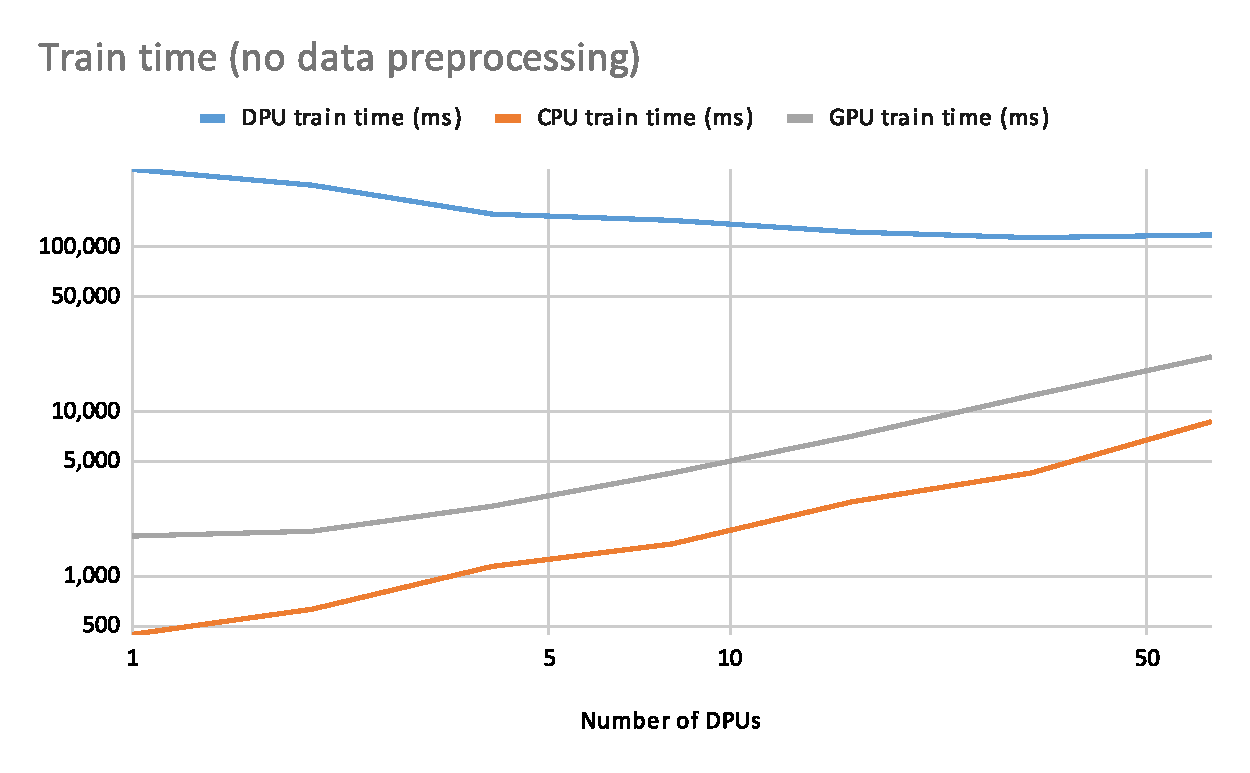
\includegraphics[width=\linewidth]{figures/KMeansweak.pdf}
        \caption{Weak scaling running times for 1 to 64 DPUs}
        \label{fig:KMeansweak}
    \end{subfigure}
    \begin{subfigure}{0.48\linewidth}
        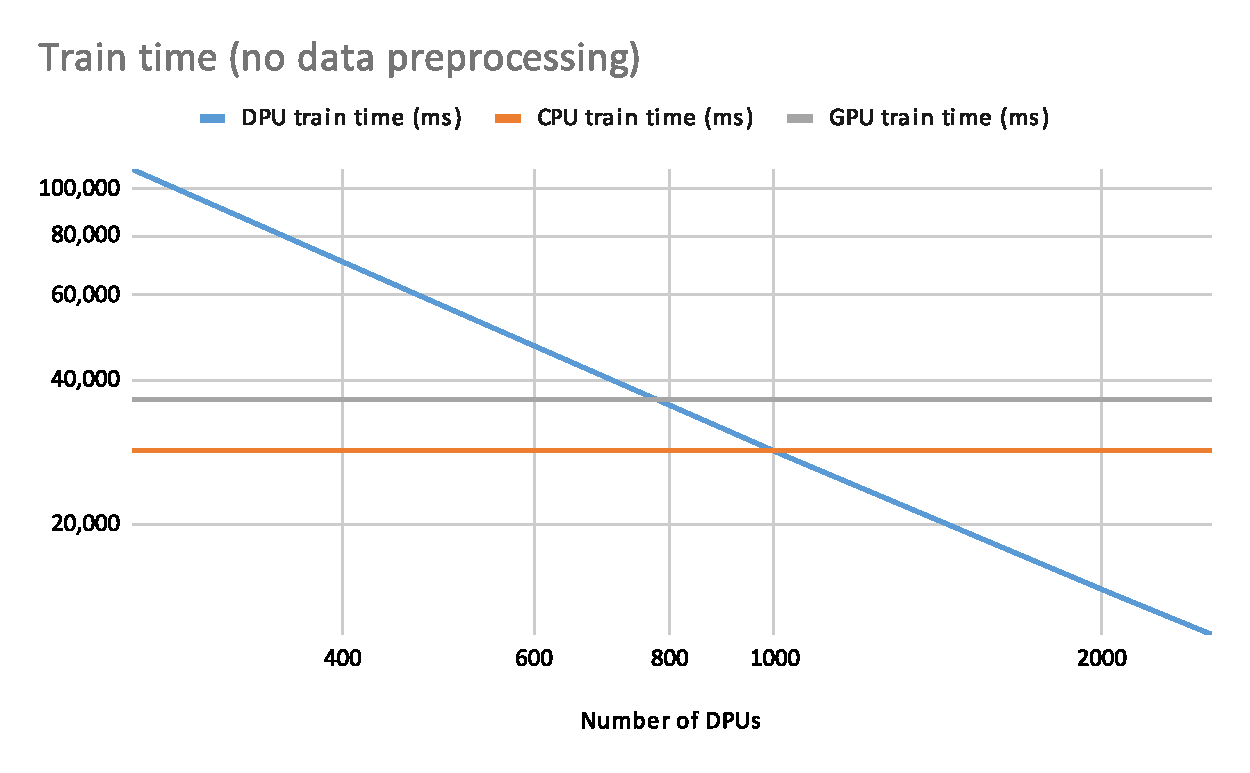
\includegraphics[width=\linewidth]{figures/KMeansstrong.pdf}
        \caption{Strong scaling running times for 256 to 2524 DPUs}
        \label{fig:KMeansstrong}
    \end{subfigure}
\end{figure}

A weak scaling test means that we scale the number of DPUs, and we also scale the dataset size so that the number of points per DPU remains constant.

The results compared to CPU and GPU can be seen on Figure \ref{fig:KMeansweak}. We can see that the processing time remains almost constant with the number of DPUs. It even reduces a little, but that's because K-Means converges in few iterations on smaller datasets. The time per iteration (not shown here) remains perfectly constant.

\subsubsection{Strong scaling}

A strong scaling test means that we scale the number of DPUs, but keep the size of the dataset constant.

The results can be seen on Figure \ref{fig:KMeansstrong}. We can see that we get a perfectly linear scaling of the performance with the number of used DPUs, surpassing the CPU at 1000 DPUs. We can also notice that the GPU is slower than the CPU. It happens on some datasets, depending on their geometry. This is due to the fact that the GPU implementation of K-Means in RAPIDS is batched for internal memory reasons, and thus less numerically stable.

